\chapter{Solomonoff Induction}

\vspace{1em}
\hfill
\begin{minipage}[c]{0.55\textwidth}
\raggedleft
\small\itshape
The only really satisfactory definition of randomness was given by Kolmogorov.\\[0.5em]
\upshape\footnotesize Gregory Chaitin, \textit{Algorithmic Information Theory} (1987)
\end{minipage}%
\hspace{0.5em}
\begin{minipage}[c]{0.12\textwidth}
% \includegraphics[width=\textwidth]{figures/ch04_solomonoff.png}
\end{minipage}
\vspace{1.5em}

\noindent The previous chapter ended with a question. Description length and probability are coupled. Different description languages give different priors. To pick a unique prior, we need a description language with a claim to universality.

This chapter introduces it. The description language is computer programs.

The result, after we work through what this means, is the universal prior $M(x)$: the prior that closes the hole Bayes left, in a sense the chapter will make precise.

\section*{Programs as descriptions}

A computer program is a description of a computation. Run it; it produces output. The output is what the program describes.

If you want to describe a particular bit string (the coin sequences of the previous chapters are an example, with heads and tails recorded as zeros and ones; so are any other binary data you might encounter), you can write a program that outputs it. There are many such programs. A trivial one: \texttt{print "01001\ldots"} with the string written out in full. A clever one: \texttt{print the first 100 binary digits of pi}. If the string in question \emph{is} the first 100 binary digits of pi, the clever program is much shorter than the trivial one.

For any string, the most efficient description is the shortest program that produces it. This length is called the \emph{Kolmogorov complexity} of the string, written $K(x)$:

$$K(x) = \text{the length, in bits, of the shortest program that outputs } x.$$

A string with regularity (the digits of pi, a repeating pattern, the text of a familiar sentence) has small $K(x)$: a short program captures the regularity. A random-looking string has $K(x)$ roughly equal to its own length: no program shorter than ``print this string'' will do.

So the description language ``computer programs'' has a natural length function, and the lengths reflect how compressible the strings are.

\section*{The library of programs}

The set of all programs is easy to describe. A program is a finite string of bits. So the set of all programs is $\{0, 1\}^*$: every finite binary string.

This set is large but trivially enumerable. Start with all strings of length one (just ``0'' and ``1''), then all strings of length two, and so on. Figure~\ref{fig:program-tree} shows the structure.

\begin{figure}[h]
\centering
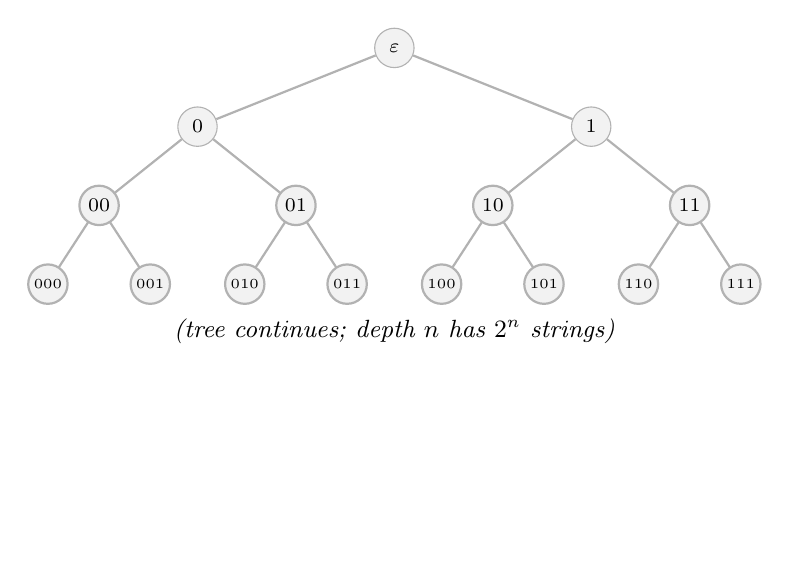
\begin{tikzpicture}[
  level distance=1cm,
  level 1/.style={sibling distance=5cm},
  level 2/.style={sibling distance=2.5cm},
  level 3/.style={sibling distance=1.3cm},
  edge from parent/.style={draw, thick, gray!60},
  every node/.style={circle, draw=gray!60, fill=gray!10, inner sep=1pt, minimum size=5mm, font=\scriptsize}
]
  \node {$\varepsilon$}
    child {node {0}
      child {node {00}
        child {node[font=\tiny] {000}}
        child {node[font=\tiny] {001}}
      }
      child {node {01}
        child {node[font=\tiny] {010}}
        child {node[font=\tiny] {011}}
      }
    }
    child {node {1}
      child {node {10}
        child {node[font=\tiny] {100}}
        child {node[font=\tiny] {101}}
      }
      child {node {11}
        child {node[font=\tiny] {110}}
        child {node[font=\tiny] {111}}
      }
    };

  \node[draw=none, fill=none, font=\small\itshape] at (0, -3.6) {(tree continues; depth $n$ has $2^n$ strings)};
\end{tikzpicture}
\caption{The library of all programs. Every program is a finite binary string and sits at some depth in this tree. Generation is trivial: descend the tree, taking $0$ or $1$ at each step. Most strings, considered as programs, are not valid syntax. Many of the valid ones do not halt. A vanishing fraction produce coherent output. All of them are in the library by virtue of being binary strings.}
\label{fig:program-tree}
\end{figure}

Most strings, considered as programs, do not parse. Most of the valid ones do not halt (they run forever without producing output). A vanishing fraction produce coherent output. Among those, a smaller fraction produce output matching anything you might be interested in. But every coherent output is in there. Every program that ever has been written is a string in this set. Every program that ever could be written is too.

\section*{The universal Turing machine}

We need one more ingredient: a machine that takes any program and runs it.

In 1936, Alan Turing showed that such a machine exists. He called it a universal machine. Given any program (any sequence of bits, encoded under a standard scheme), the universal machine runs that program and produces the corresponding output.

In modern language: every computer is a universal machine. Your laptop, given any program in a language it can read, runs it. The universality is mathematical: anything computable by any computer is computable by every computer, up to a constant factor in description length and time. Different computers differ in speed and convenience but not in what they can compute.

We will use $U$ to refer to such a universal machine. The choice of $U$ is conventional. Different universal machines exist, but for our purposes they are interchangeable: anything you can do on machine $U_1$, you can do on machine $U_2$ with a small extra cost (the cost of a translator program from one to the other). This is the \emph{invariance theorem}, and it is why the results below do not depend critically on the choice of $U$.

\section*{The universal prior}

Now we put the pieces together.

Take any string $x$ you might want to predict, or describe, or weight. Consider all the programs that produce $x$ when run on $U$. There are many. Each has a length $|p|$, its size in bits.

The universal prior $M(x)$ is

$$M(x) = \sum_{p \,:\, U(p) = x\star} 2^{-|p|}.$$

The sum is over all programs $p$ such that $U(p)$ produces $x$ as a prefix of its output (the star denotes ``with possibly more after''). Each program contributes weight $2^{-|p|}$. Long programs contribute little; short programs contribute a lot. Figure~\ref{fig:M-sum} shows the structure.

\begin{figure}[h]
\centering
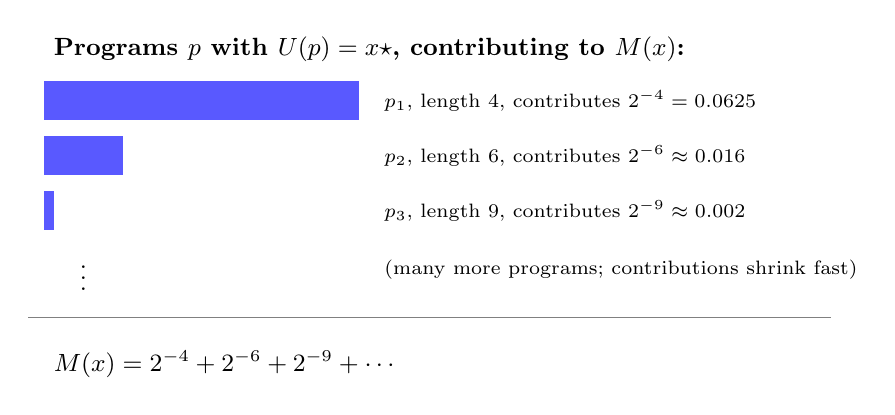
\begin{tikzpicture}[scale=1.0]
  \node[font=\small\bfseries, anchor=west] at (0, 3.4) {Programs $p$ with $U(p) = x\star$, contributing to $M(x)$:};

  % p1 length 4, width 4
  \fill[blue!65] (0, 2.5) rectangle (4, 3.0);
  \node[font=\scriptsize, anchor=west] at (4.2, 2.75) {$p_1$, length 4, contributes $2^{-4} = 0.0625$};

  % p2 length 6, width 1
  \fill[blue!65] (0, 1.8) rectangle (1, 2.3);
  \node[font=\scriptsize, anchor=west] at (4.2, 2.05) {$p_2$, length 6, contributes $2^{-6} \approx 0.016$};

  % p3 length 9, width 1/8
  \fill[blue!65] (0, 1.1) rectangle (0.125, 1.6);
  \node[font=\scriptsize, anchor=west] at (4.2, 1.35) {$p_3$, length 9, contributes $2^{-9} \approx 0.002$};

  % dots
  \node[font=\small] at (0.5, 0.6) {$\vdots$};
  \node[font=\scriptsize, anchor=west] at (4.2, 0.6) {(many more programs; contributions shrink fast)};

  \draw[gray, thin] (-0.2, 0.0) -- (10, 0.0);
  \node[font=\small, anchor=west] at (0, -0.6) {$M(x) = 2^{-4} + 2^{-6} + 2^{-9} + \cdots$};
\end{tikzpicture}
\caption{The universal prior $M(x)$ as a sum. Every program $p$ that produces $x$ as a prefix of its output contributes $2^{-|p|}$ to $M(x)$. The shortest such program has length $K(x)$ and contributes the dominant term. Strings with short descriptions are heavy. Strings without are light.}
\label{fig:M-sum}
\end{figure}

This is Kraft taken to its limit. The description language is ``programs for $U$.'' The lengths are program lengths. The implied probability over outputs is $M(x)$.

\subsection*{What $M$ inherits from Kraft}

A standard technical setup gives $U$ a self-delimiting input convention: each program signals its own end as it is read, so the set of valid programs is prefix-free.\footnote{For the continuous-output formulation used here (programs producing $x$ as a prefix of their output), the conventional setup is a \emph{monotone} Turing machine. A different but related setup, the prefix Turing machine, gives the discrete formula $m(x) = \sum_{p\,:\,U(p)=x} 2^{-|p|}$. Both setups give Kraft-style bounds; the qualitative properties of $M$ in this chapter hold in either.} Kraft then guarantees that the total weight is bounded: $\sum_x M(x) \leq 1$. The universal prior is well-defined.

\subsection*{What $M$ inherits from programs}

A string with low $K(x)$ has at least one short program producing it. That short program contributes $2^{-K(x)}$ to the sum. So

$$M(x) \geq 2^{-K(x)}.$$

For most $x$, this bound is nearly tight: the description length $-\log_2 M(x)$ equals $K(x)$ to within a term that grows only logarithmically in $K(x)$. The universal prior is, up to that lower-order correction in the exponent, the exponential of the negative Kolmogorov complexity. Compressible things are probable; incompressible things are improbable.

Occam's razor falls out of this. Simpler hypotheses (shorter programs) get higher prior weight, not by stipulation but as a structural consequence of using programs as the description language.

\section*{Solomonoff induction}

Given the universal prior, Bayesian inference proceeds in the usual way. Suppose you observe data $x$. To predict whether the next bit is $0$ or $1$, you compute the conditional:

$$M(\text{next bit} = b \mid x) = \frac{M(xb)}{M(x)}.$$

This is what \emph{Solomonoff induction} refers to: Bayesian inference using $M$ as the prior. Given any history of observations, the predictor's belief about the next observation is well-defined. Update as new observations come in. The procedure is recursive, principled, and parameter-free.

Solomonoff defined this in the 1960s. The puzzle of where the prior comes from, which had bedeviled Bayesian inference for two centuries, was answered by a particular choice that does not look arbitrary: the prior weighted by program lengths.

\section*{The dominance theorem}

Now the result that makes $M$ optimal.

Suppose there is some true probability distribution $\mu$ generating your data. You do not know $\mu$. You want to predict the data, hoping your prior is close enough to $\mu$ to be useful.

The dominance theorem says: if $\mu$ is computable (or, more precisely, lower-semicomputable as a semimeasure), then there is a constant $c_\mu$ such that

$$M(x) \geq c_\mu \cdot \mu(x) \text{ for every } x.$$

In words: $M$ never assigns much less weight to any sequence than $\mu$ does. The ratio $M(x) / \mu(x)$ is bounded below by a constant that depends on $\mu$ but not on $x$. Figure~\ref{fig:dominance} shows the envelope.

\begin{figure}[h]
\centering
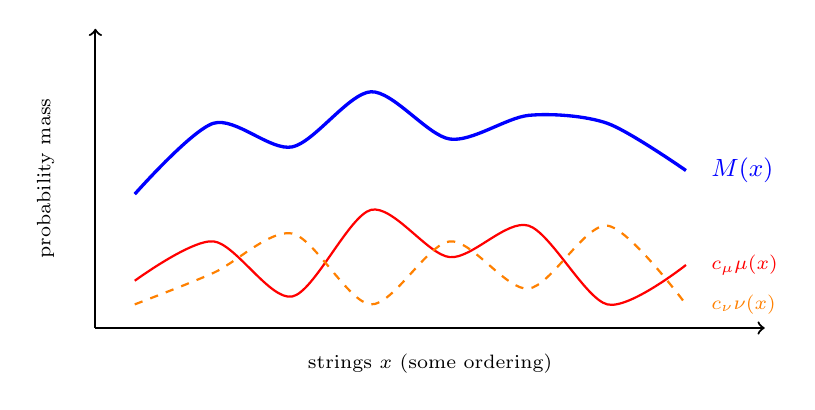
\begin{tikzpicture}[scale=1.0]
  \draw[->, thick] (0, 0) -- (8.5, 0);
  \draw[->, thick] (0, 0) -- (0, 3.8);
  \node[font=\scriptsize, anchor=north] at (4.25, -0.2) {strings $x$ (some ordering)};
  \node[font=\scriptsize, rotate=90, anchor=south] at (-0.4, 1.9) {probability mass};

  % mu(x) scaled by c_mu - lower curve, red
  \draw[red, thick] plot[smooth, tension=0.5] coordinates {(0.5, 0.6) (1.5, 1.1) (2.5, 0.4) (3.5, 1.5) (4.5, 0.9) (5.5, 1.3) (6.5, 0.3) (7.5, 0.8)};
  \node[red, font=\scriptsize, anchor=west] at (7.7, 0.8) {$c_\mu \mu(x)$};

  % nu(x) scaled by c_nu - another lower curve, orange
  \draw[orange, thick, dashed] plot[smooth, tension=0.5] coordinates {(0.5, 0.3) (1.5, 0.7) (2.5, 1.2) (3.5, 0.3) (4.5, 1.1) (5.5, 0.5) (6.5, 1.3) (7.5, 0.3)};
  \node[orange, font=\scriptsize, anchor=west] at (7.7, 0.3) {$c_\nu \nu(x)$};

  % M(x) - upper envelope, blue
  \draw[blue, very thick] plot[smooth, tension=0.5] coordinates {(0.5, 1.7) (1.5, 2.6) (2.5, 2.3) (3.5, 3.0) (4.5, 2.4) (5.5, 2.7) (6.5, 2.6) (7.5, 2.0)};
  \node[blue, font=\small\bfseries, anchor=west] at (7.7, 2.0) {$M(x)$};
\end{tikzpicture}
\caption{The dominance theorem. $M(x)$ (blue, thick) lies above every computable distribution after appropriate scaling. For each computable distribution $\mu$, there exists a constant $c_\mu$ such that $M(x) \geq c_\mu \cdot \mu(x)$ for all $x$. The constants depend on the distribution but not on $x$. As data accumulates, the predictions of $M$ converge to the true distribution.}
\label{fig:dominance}
\end{figure}

Equivalently: the predictions of $M$ converge to the predictions of $\mu$ as data accumulates.\footnote{This convergence is quantitative and fast. The total expected Kullback-Leibler divergence between $\mu$ and $M$, summed over all steps, is bounded by the description length of $\mu$: $\sum_{t=1}^{\infty} \mathbb{E}_\mu\!\left[\mathrm{KL}\big(\mu(\cdot \mid x_{<t}) \,\|\, M(\cdot \mid x_{<t})\big)\right] \leq K(\mu)\ln 2$ (Hutter 2001, 2005). Because the bound is finite and independent of sequence length, the per-step divergence must fall to zero: $M$'s predictions converge to $\mu$'s, and the cumulative cost of not having known $\mu$ in advance is at most $K(\mu)\ln 2$ nats.} After enough observations, $M$ and $\mu$ make essentially the same predictions about what comes next, regardless of which $\mu$ is at work.

The result has wide reach. It does not say $M$ is the true distribution. It says: \emph{whatever} the true computable distribution is, $M$ will converge to it. $M$ is contained inside every computable distribution, up to a constant.

This is what optimal induction looks like. You do not need to know what is generating the data. You weight your hypotheses by program length, sum them as $M$, and your predictions converge to whatever computable process is actually at work.

\section*{The catch}

$M$ is uncomputable.

To compute $M(x)$ exactly, you would need to enumerate every program that produces $x$ as a prefix of its output and sum their $2^{-|p|}$ contributions. There are infinitely many such programs. Worse, you cannot tell in advance which programs halt (the halting problem); for any given program, you cannot decide whether it will eventually produce $x$ or run forever without doing so.

You can approximate $M(x)$ from below. Run all programs up to some length, for some number of steps, and sum the contributions of the ones that have produced $x$ by then. The approximation improves monotonically with more time. But there is no finite procedure that gives $M(x)$ exactly, and no way to know how close your approximation is.

This is not a flaw in the definition. It is what makes $M$ universal. Any prior you could compute exactly would be simpler in some way than the universal one, and would fail dominance against the priors it could not capture.

The result: $M$ is the right reference point for what optimal induction is. No actual inductor (biological or mathematical or machine) computes $M$. Every actual inductor is an approximation, faster but coarser.

This is what the rest of the book is about.

\section*{Where this leaves you}

The hole Bayes left, the choice of prior, is now closed at one level.

The unique optimal prior is $M$. It dominates every computable distribution. It realizes Occam's razor as a structural consequence of using programs as the description language. It does not depend on conventions, because invariance handles the choice of $U$.

The cost: $M$ cannot be computed. Any practical inductor approximates it.

Two strands follow.

\textbf{Theoretical.} What does an optimal agent look like? Solomonoff induction is the prediction half. The next four chapters add the decision half: how an optimal agent uses predictions to choose actions. The synthesis is called AIXI.

\textbf{Practical.} How do real systems approximate optimal induction? They do not run $M$ or anything resembling it directly. They use bounded methods that work in practice. Large language models are one important example. Part IV of the book is about what these systems actually do and how they relate (or fail to relate) to the reference point that $M$ provides.\footnote{There is also a philosophical thread the mathematics raises but does not settle: if the shortest program that fits your observations is the best explanation of them, what does the library of all programs say about where those observations come from? \emph{A Philosophical Note} at the back of the book follows that question as far as it honestly goes, and no further.}

Part I closes here. The next chapter takes the first step toward agency: the decision problem. If you can predict, how should you act? That is where Part II begins.
